%%%%%%%%%%%%%%%%%%%%%%%%%%%%%%%%%%%%%%%%%%%%%%%%%%%%%%%%%%%%%%%%%%%%%%%%%%%%%%%%
% Template for USENIX papers.
%
% History:
%
% - TEMPLATE for Usenix papers, specifically to meet requirements of
%   USENIX '05. originally a template for producing IEEE-format
%   articles using LaTeX. written by Matthew Ward, CS Department,
%   Worcester Polytechnic Institute. adapted by David Beazley for his
%   excellent SWIG paper in Proceedings, Tcl 96. turned into a
%   smartass generic template by De Clarke, with thanks to both the
%   above pioneers. Use at your own risk. Complaints to /dev/null.
%   Make it two column with no page numbering, default is 10 point.
%
% - Munged by Fred Douglis <douglis@research.att.com> 10/97 to
%   separate the .sty file from the LaTeX source template, so that
%   people can more easily include the .sty file into an existing
%   document. Also changed to more closely follow the style guidelines
%   as represented by the Word sample file.
%
% - Note that since 2010, USENIX does not require endnotes. If you
%   want foot of page notes, do not include the endnotes package in the
%   usepackage command, below.
% - This version uses the latex2e styles, not the very ancient 2.09
%   stuff.
%
% - Updated July 2018: Text block size changed from 6.5" to 7"
%
% - Updated Dec 2018 for ATC'19:
%
%   * Revised text to pass HotCRP's auto-formatting check, with
%     hotcrp.settings.submission_form.body_font_size=10pt, and
%     hotcrp.settings.submission_form.line_height=12pt
%
%   * Switched from \endnote-s to \footnote-s to match Usenix's policy.
%
%   * \section* => \begin{abstract} ... \end{abstract}
%
%   * Make template self-contained in terms of bibtex entires, to allow
%     this file to be compiled. (And changing refs style to 'plain'.)
%
%   * Make template self-contained in terms of figures, to
%     allow this file to be compiled. 
%
%   * Added packages for hyperref, embedding fonts, and improving
%     appearance.
%   
%   * Removed outdated text.
%
%%%%%%%%%%%%%%%%%%%%%%%%%%%%%%%%%%%%%%%%%%%%%%%%%%%%%%%%%%%%%%%%%%%%%%%%%%%%%%%%

\documentclass[letterpaper,twocolumn,10pt]{article}
\usepackage{usenix2019_v3}

% to be able to draw some self-contained figs
\usepackage{tikz}
\usepackage{amsmath}

% inlined bib file
\usepackage{filecontents}

\usepackage{listings}
\usepackage{parcolumns}
\usepackage{graphicx}
\usepackage{caption}
\usepackage{subcaption}
\usepackage{cleveref}

%-------------------------------------------------------------------------------
\begin{filecontents}{\jobname.bib}
%-------------------------------------------------------------------------------
@book{silberschatz2018operating,
  title={Operating system principles},
  author={Silberschatz, Abraham and Galvin, Peter Baer and Gagne, Greg},
  year={2018},
  publisher={John Wiley \& Sons},
  edition={10}
}

@article{watson2007exploiting,
  title={Exploiting Concurrency Vulnerabilities in System Call Wrappers.},
  author={Watson, Robert NM},
  journal={WOOT},
  volume={7},
  pages={1--8},
  year={2007}
}

@inproceedings{wang2017double,
  title={How double-fetch situations turn into double-fetch vulnerabilities: A 
  study of double fetches in the linux kernel},
  author={Wang, Pengfei and Krinke, Jens and Lu, Kai and Li, Gen and 
  Dodier-Lazaro, Steve},
  booktitle={26th $\{$USENIX$\}$ Security Symposium 
  ($\{$USENIX$\}$ Security 17)},
  pages={1--16},
  year={2017}
}

@inproceedings{schwarz2018automated,
  title={Automated detection, exploitation, and elimination of double-fetch bugs
   using modern CPU features},

  author={Schwarz, Michael and Gruss, Daniel and Lipp, Moritz and Maurice,
  Cl{\'e}mentine and Schuster, Thomas and Fogh, Anders and Mangard, Stefan},

  booktitle={Proceedings of the 2018 on Asia Conference on Computer and Communications Security},
  pages={587--600},
  year={2018}
}

@inproceedings{xu2018precise,
  title={Precise and scalable detection of double-fetch bugs in OS kernels},
  author={Xu, Meng and Qian, Chenxiong and Lu, Kangjie and Backes, Michael
   and Kim, Taesoo},
  booktitle={2018 IEEE Symposium on Security and Privacy (SP)},
  pages={661--678},
  year={2018},
  organization={IEEE}
}

@article{wang2018survey,
  title={A survey of the double-fetch vulnerabilities},
  author={Wang, Pengfei and Lu, Kai and Li, Gen and Zhou, Xu},
  journal={Concurrency and Computation: Practice and Experience},
  volume={30},
  number={6},
  pages={e4345},
  year={2018},
  publisher={Wiley Online Library}
}

@article{jurczyk2013bochspwn,
  title={Bochspwn: Identifying 0-days via system-wide memory access pattern analysis},
  author={Jurczyk, GC Mateusz and Coldwind, Gynvael},
  journal={Black Hat USA Briefings (Black Hat USA)},
  year={2013}
}


@article{lu2018untrusted,
  title={Untrusted hardware causes double-fetch problems in the I/O memory},
  author={Lu, Kai and Wang, Peng-Fei and Li, Gen and Zhou, Xu},
  journal={Journal of Computer Science and Technology},
  volume={33},
  number={3},
  pages={587--602},
  year={2018},
  publisher={Springer}
}

@inproceedings{payer2012protecting,
  title={Protecting applications against TOCTTOU races by user-space caching of file metadata},
  author={Payer, Mathias and Gross, Thomas R},
  booktitle={Proceedings of the 8th ACM SIGPLAN/SIGOPS conference on Virtual Execution Environments},
  pages={215--226},
  year={2012}
}

@inproceedings{pu2006methodical,
  title={A methodical defense against tocttou attacks: The edgi approach},
  author={Pu, Calton and Wei, Jinpeng},
  booktitle={Proceedings of the 2006 International Symposium on Secure Software Engineering},
  year={2006}
}

@article{wei2010modeling,
  title={Modeling and preventing TOCTTOU vulnerabilities in Unix-style file systems},
  author={Wei, Jinpeng and Pu, Calton},
  journal={computers \& security},
  volume={29},
  number={8},
  pages={815--830},
  year={2010},
  publisher={Elsevier}
}

@inproceedings{tsafrir2008portably,
  title={Portably Solving File TOCTTOU Races with Hardness Amplification.},
  author={Tsafrir, Dan and Hertz, Tomer and Wagner, David A and Da Silva, Dilma},
  booktitle={FAST},
  volume={8},
  pages={1--18},
  year={2008}
}

@misc{zak_frasunek_dawidek,
  title={CerbNG},
  url={https://sourceforge.net/projects/cerber/files/cerb-ng/}, 
  journal={CerbNG}, 
  author={Zak, Slawek and Frasunek, Przemyslaw and Dawidek, Pawel Jakub}
} 

@misc{seccomp,
  title={SecComp},
  url={https://www.kernel.org/doc/html/latest/userspace-api/seccomp_filter.html}, 
} 

@misc{ebpf,
  title={eBPF},
  url={https://lwn.net/Articles/740157/}, 
}

@misc{landlock,
  title={Landlock LSM},
  url={https://landlock.io/},
  author={Mickaël Salaün}
}

@misc{krsi,
  title={Kernel Runtime Security Instrumentation},
  url={https://github.com/sinkap/linux-krsi},
  author={K. P. Singh}
}

@inproceedings{morris2002linux,
  title={Linux security modules: General security support for the linux kernel},
  author={Morris, James and Smalley, Stephen and Kroah-Hartman, Greg},
  booktitle={USENIX Security Symposium},
  pages={17--31},
  year={2002},
  organization={ACM Berkeley, CA}
}

@article{smalley2001implementing,
  title={Implementing SELinux as a Linux security module},
  author={Smalley, Stephen and Vance, Chris and Salamon, Wayne},
  journal={NAI Labs Report},
  volume={1},
  number={43},
  pages={139},
  year={2001}
}

@misc{gruenbacher2007apparmor,
  title={AppArmor Technical Documentation},
  author={Gruenbacher, Andreas and Arnold, Seth},
  year={2007}
}

@article{intel64and,
  title={Intel 64 and IA-32 Architectures Developer's Manual},
  author={{Intel}},
  chapter={Programming with Intel® Transactional Synchronization Extensions},
  volume={1},
  chapter={16},
  year={2019}
}



\end{filecontents}

%-------------------------------------------------------------------------------
\begin{document}
%-------------------------------------------------------------------------------

%do not want date printed
\date{}

% make title bold and 14 pt font (Latex default is non-bold, 16 pt)
\title{\Large \bf TikTok: Kernel TOCTTOU Protection}

%for single author (just remove % characters)
\author{
{\rm Uro\v{s} Te\v{s}i\'{c}}\\
EPFL
\and
{\rm Mathias Payer}\\
EPFL
% copy the following lines to add more authors
% \and
% {\rm Name}\\
%Name Institution
} % end author

\maketitle

%-------------------------------------------------------------------------------
\begin{abstract}
%-------------------------------------------------------------------------------
Your abstract text goes here. Just a few facts. Whet our appetites.
Not more than 200 words, if possible, and preferably closer to 150.
\end{abstract}

% Talk about the system call filters and how they can be used for good
% Introduce the main problem - TOCTTOU
% Brag how our system is the best thing since sliced bread
\section{Introduction}
System call wrappers enable administrators to define system call execution
policies. Such policies could prevent the execution of a system call based 
on the ID of the call and its arguments. By setting only necessary access
policies for all processes, administrators would reduce the damage in case 
of an attack. Filtering could also restrict calls to the exploitable system
calls. By excluding some combinations of arguments, the administrator could 
mitigate certain vulnerabilities until a patch is available. Many embedded 
devices have binary-only drivers that prevent them from updating the 
kernel. Malicious input filtering could be used as a permanent solution in 
those cases.
\\
\\
Unfortunately, system call wrappers suffer from a design flaw. Filters execute 
before system calls. After the filter reads arguments and validates them, the
system call reads them the second time. In-between these two reads, the attacker
could change values, leading to an execution of a forbidden call. This is called
a \emph{time-of-check to time-of-use} attack (TOCTTOU). It is a consequence of a
\emph{double fetch} from the userland and is notoriously hard to detect. Unlike 
other bugs, double-fetches are benign until the adversary decides to change the 
arguments.
\\
\\
\begin{figure}[]
  \centering
  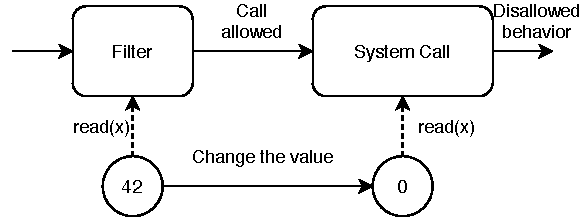
\includegraphics[width=.85\linewidth]{img/tocttou.pdf}
  \caption{Bypassing a system call filter using a TOCTTOU attack}
  \label{fig:tocttou}
\end{figure}

The contributions of this paper are:
\begin{itemize}
\item TikTok - mitigation for time-of-check to time-of-use attacks on system 
      call arguments in the Linux kernel
\item A technique to postpone the writes from userland
\item A technique to defer the writes from the kernel, while continuing normal
      kernel execution
\item Performance analysis of our system and its security guarantees
\end{itemize}

The rest of the paper is organized as follows: \Cref{sec:background} explains 
inter-process communication, paging, double fetch bugs, and the related
background. \Cref{sec:design} describes how \emph{TikTok} works in theory, while
\cref{sec:implementation} elaborates on the x86-64 implementation. Related work
is discussed in \cref{sec:relatedwork}.

% Cover the theory needed to understand how and why TikTok works
% 1) IPC - We need this to argue why the deadlocks are almost impossible
% 2) VM and Page Tables - Why it exists and how it works
% 3) x86 Page Tables - Continue the discussion from the previous section
% 4) Page faults - Explain how and why they happen.
\section{Background}

\label{sec:background}
\subsection{Interprocess Communication}

The two main types of communication between processes are \emph{shared memory} 
and \emph{message passing}\cite{silberschatz2018operating}.
\\
\\
Shared memory relies on processes having a section of memory that both can 
access. Data transfer is fast. However, synchronization is problematic. 
Processes must monitor shared memory for changes, leading to unnecessary
polling.
\\
\\
Message passing consists of one process calling send, and another one calling
receive to fetch the message. Synchronization is guaranteed, with parties
waiting for their calls to be served. However, unnecessary message copying can
occur between processes on the same system.
\\
\\
Modern operating systems support both of these approaches. The downsides are
usually offset by adding the  bare minimum of the other approach (e.g. shared
memory with semaphores, or message passing with shared buffers). Two processes
usually use only one paradigm to communicate. Sending messages and writing
to the shared memory at the same time is exceptionally rare.

\subsection{Virtual Memory and Page Tables} \label{sec:vm}

Operating system (OS) provides an illusion that every process is executing alone
on the processor. To accomplish this, the OS needs to restore the program state
on the context switch between two processes (e.g. CPU registers) and to prevent 
processes from accessing each other's memory. Memory is protected by
\emph{virtualization}. Processes use \emph{virtual addresses} that get mapped to
the \emph{physical addresses}. When the OS moves data to a different physical 
address, the virtual address referring to the data remains the same.
\\
\\
Virtual memory can be implemented by storing different processes' data at 
different offsets in physical memory and limiting the access to corresponding 
memory chunks. Each process's memory chunk is called a segment and the 
implementation is called \emph{segmented virtual memory}. The translation is 
accomplished by adding an offset to the virtual address. Considering that 
segments need to be continuous, the free physical memory can be fragmented
such that the OS cannot find a part large enough to store a new process.
\\
\\
\begin{figure}

  \begin{subfigure}[]{.45\linewidth}
    \centering
    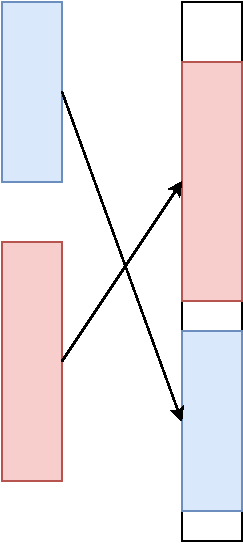
\includegraphics[width=.5\linewidth]{img/segmented.pdf}
    \caption{Segmented}
  \end{subfigure}
  \hfill
  \begin{subfigure}[]{.45\linewidth}
    \centering
    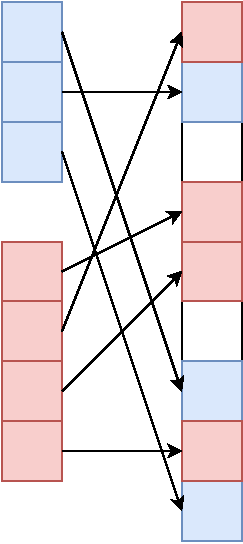
\includegraphics[width=.5\linewidth]{img/paged.pdf}
    \caption{Paged}
  \end{subfigure}

  \caption{Two virtual memory spaces mapped to physical memory using segmented
  and paged approaches}
\end{figure}

\emph{Paged virtual memory} is more flexible. The physical memory is partitioned
into fixed-size pages (usually 4 kB). A page in the virtual memory space gets
mapped to the corresponding page in the physical memory. The mapping function is
defined for each process by a \emph{page-table}. Page-tables store the reference
to the mapped physical memory (\emph{page frame}). They also keep
the access permissions for each page (\emph{read}, \emph{write}, \emph{execute},
 \emph{user}, \emph{superuser}). In case of low memory, rarely accessed pages 
can be moved to the disk, and replaced by immediately needed pages. This process
is called \emph{swapping}. Similarly, when processing a file, pages do not need 
to be loaded immediately, but on the first access (\emph{on-demand paging}). The
\emph{present} bit is added to differentiate between present and absent pages.
\\
\\
Virtual memory spaces are quite large ($2^{64}$ bytes on a 64-bit processor). A 
table containing all one-to-one mappings would be impossibly large to store. 
Page tables are therefore stored as trees with only the allocated memory being 
present (\cref{fig:pagetable}). However, instead of just reading the 
corresponding physical address on memory access, the processor now needs to 
perform a tree traversal. Different bits in a virtual address encode the path 
the processor needs to take to obtain the page frame number (e.g. the first 8 
bits tell CPU which entry on the first level it needs to dereference). Traversal
needs to be fast. It is implemented in hardware by the \emph{memory management 
unit} (MMU). Reading the page table from memory is slow, so a small cache is 
added to the MMU to store frequently accessed page entries - 
\emph{translation-lookaside buffer} (TLB). On modern processors, TLB consists of
several levels, and can even be backed by another MMU cache. 

\subsection{x86-64 Page Tables}

\begin{figure}[]
  \centering
  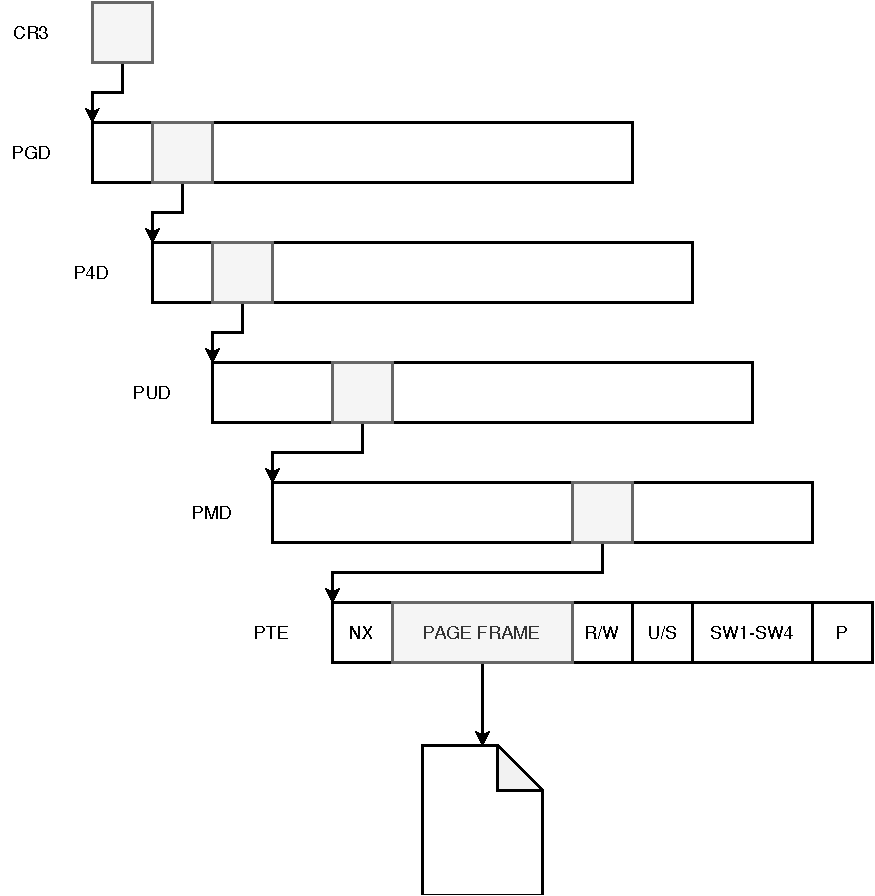
\includegraphics[width = .35 \textwidth]{img/pagetable.pdf}
  \caption{Page Table Structure on x86. Only relevant data has been included.}
  \label{fig:pagetable}
\end{figure}
x86-64 architecture officially supports paged virtual memory model with a 5 
level page table (\cref{fig:pagetable}):
\begin{description}
    \item[PGD] Page Global Directory
    \item[P4D] Page Fourth-level Directory
    \item[PUD] Page Upper Directory
    \item[PMD] Page Middle Directory
    \item[PTE] Page Table Entry
\end{description}

Every level corresponds to 8 bits in the virtual address, with the remaining 12
bits identifying the offset in the actual page frame. A page table entry
includes the following information:
\begin{description}
    \item[Present bit (\textbf{P})] is set if the page is present in memory
    \item[Read/Write bit (\textbf{R/W})] denotes if the page is writable or just
         readable
    \item[User/Superuser bit (\textbf{U/S})] represents if the page can be 
    accessed by the user, or only by the superuser
    \item[Not Executable bit (\textbf{NX})] is set if the code stored on the 
    page cannot be executed
    \item[Page Frame Number] denotes the page frame the entry points to
    \item[\textbf{SW1-SW4}] Four bits free for the OS to use
\end{description}

\subsection{Page-Faults}
On invalid access (e.g. wrong permissions, page not present) the MMU will 
trigger a page-fault. The fault is a synchronous interrupt that executes in the 
context of the faulting (accessing) thread. The page-fault handler loads an 
absent page from the disk. In the case of a write to a temporarily shared page,
it creates an independent copy of the page (\emph{copy-on-write}). On permission
iolation, the page-fault handler kills the thread. After the fault finishes
executing, the faulting instruction is re-executed. 
\\
\\
With the advent of cloud computing, userland page-fault handling has been added 
to the Linux kernel. Users can define their routines to load swapped-out data.
This is particularly useful on computer farms when migrating virtual machines
between physical nodes. One only needs to migrate the code that is executing.
Accesses to the unmigrated memory will be passed to the userland page-fault
handler. It will then fetch them over the network and continue the execution.

\subsection{Copy-from-User and Copy-to-User}
Linux uses swapping only for user memory. When executing in the kernel context,
kernel memory is mapped and present. A page fault on kernel memory access is
therefore considered fatal. However, the kernel needs to access potentially
paged-out user memory. The user memory is also limited to the lower half of the
virtual memory space. On every access to the user-pointer, the kernel needs to
verify this constraint.
\\
\\
Linux provides functions and macros for user-memory access from the kernel to 
enforce the checks. A page-fault generated by them is treated as a fault in the
user process which had invoked the executing system call.
\\
\\
The interface for communication with userspace:
\begin{itemize}
    \item[] \texttt{copy\_(from/to)\_user}
    \item[] \texttt{\_\_copy\_(from/to)\_user}
    \item[] \texttt{(get/put)\_user}
    \item[] \texttt{\_\_(get/put)\_user}
    \item[] \texttt{user\_strcpy}
    \item[] \texttt{user\_strlen}
\end{itemize}
\bigskip
BSD also provides a similar interface using \texttt{copy\_in} and 
\texttt{copy\_out} functions.

\subsection{Double Fetch Bugs}

\label{subsec:doublefetch}

\begin{figure}[]
  \centering
  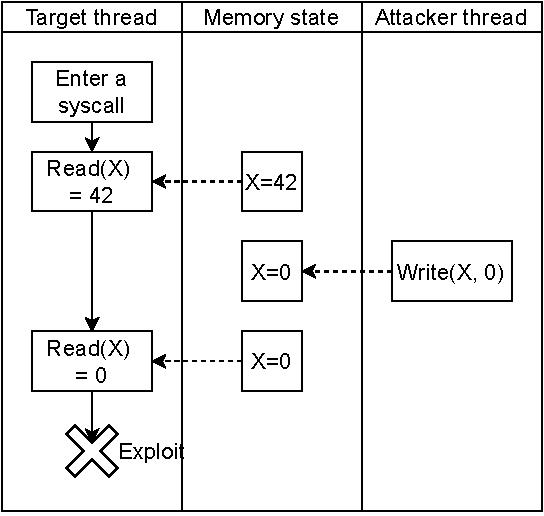
\includegraphics[width=.85\linewidth]{img/doublefetch.pdf}
  \caption{Diagram of a double fetch bug}
  \label{fig:doublefetch}
\end{figure}

\emph{Double fetch} bugs occur when a privileged environment (such as the 
kernel) reads untrusted memory two or more times (\cref{fig:doublefetch}). 
In between those two reads, memory could have been changed by an unprivileged
adversary. Considering that this bug relies on carefully timed accesses
for two different threads, it is a variant of a race condition. The situation
where the first fetch validates the value of the fetched variable, 
but the computation is only performed on the second fetch, is called a 
\emph{time-of-check to time-of-use} (TOCTTOU) bug. TOCTTOU bugs have been
widely studied in file systems, where the API makes it possible to swap the file
after validating the access rights \cite{payer2012protecting,
pu2006methodical, wei2010modeling, tsafrir2008portably}.
\\
\\
Wang et al. explain in \cite{wang2018survey} that double fetches appear not only
in kernels, but wherever there is a trust boundary to cross (e.g. kernel -- 
hypervisor, hardware -- kernel). Double fetches have been responsible for many
vulnerabilities in the kernel.


\section{Design}
\label{sec:design}
In this section we describe a high-level overview of TikTok. We start with the 
security model in \cref{subsec:secmodel}. Afterward we describe how TikTok 
protects system call arguments from userland (\cref{subsec:userland}) and the 
kernel (\cref{subsec:kernelland}) writes.

\subsection{The Security Model}
\label{subsec:secmodel}
The administrator has set up DAC preventing the adversary from accessing files 
mapping to physical devices. They also control which file-systems are mounted on
the machine and have disabled userland page-fault handling.
\\
\\
The adversary has access to a user account on a target machine. They can execute
arbitrary code (including system call) and want to obtain root access by 
triggering a TOCTTOU bug in the kernel.

\subsection{Protecting System Call Arguments from Writes by the User}
\label{subsec:userland}
\begin{figure}[]
  \centering
  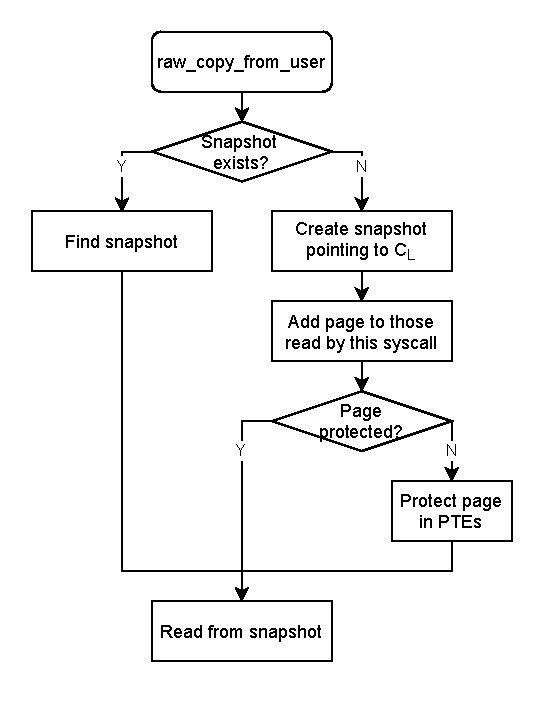
\includegraphics[width = .45 \textwidth]{img/copy_from_user.pdf}
  \caption{\texttt{copy\_from\_user} marks both the file and the pages before
  reading in the data}
  \label{fig:copyfromuser}
\end{figure}

System calls access the user memory via \texttt{copy\_from\_user} and its 
variants. When that happens, TikTok \emph{marks} the entire page storing the 
argument as \emph{read-only} in all virtual memory spaces mapping it 
(\cref{fig:copyfromuser}). Multiple system calls can mark a page at the same 
time. Marking a page does not affect readsfrom userspace in any way. When all 
the system calls that use the page finish executing, the page is \emph{unmarked}
 -- the previous permissions are restored.
\\
\\
Writes to the marked pages will trigger a page-fault (\cref{fig:pagefault}). In 
the page-fault handler we intercept these writes and make them wait for the page
to get unmarked. The faulting thread attempts to perform the write again.

\begin{figure}[]
  \centering
  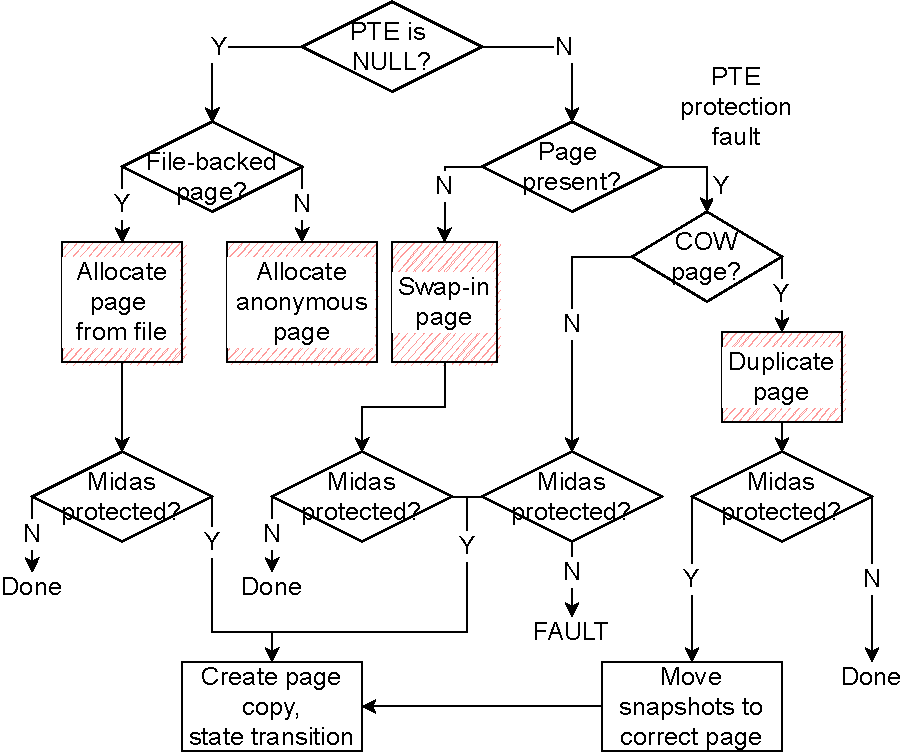
\includegraphics[width = .75 \linewidth]{img/pagefault.pdf}
  \caption{TikTok's handling of the writes to a marked page}
  \label{fig:pagefault}
\end{figure}

\subsection{Protecting System Call Aguments from Writes by the Kernel}
\label{subsec:kernelland}
\begin{figure}[]
  \centering
  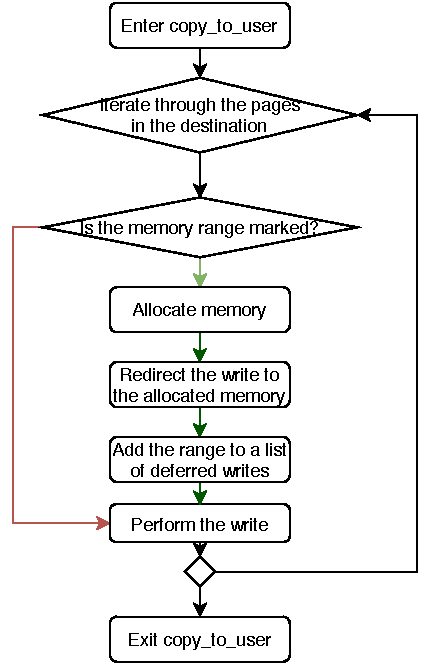
\includegraphics[width = .30 \textwidth]{img/copy_to_user.pdf}
  \caption{\texttt{copy\_to\_user} defers the writes from kernel until the end
  of the system call}
  \label{fig:copytouser}
\end{figure}

Watson mentions in \cite{watson2007exploiting} that the system call wrappers he
analyzed do not handle both reads and writes in the same call properly. Unlike
those solutions, TikTok does not copy arguments to separate memory, leading to
complex redirection of userspace pointers. TikTok defers the writes until it is
safe to commit the writes.
\\
\\
However, deferring kernel writes the same way as user writes would lead to
deadlocks. System call \texttt{rt\_sigaction} needs to write to a page it
previously marked. Pausing execution would leave the thread in a state where it
is waiting for itself to exit unmark the page. Temporarily unmarking the page
would enable an adversary to edit arbitrary data on it.
\\
\\
Allowing the writes for the kernel is not an option. The adversary could abuse
this to change the marked memory. They would execute a read system call into
the marked page. System calls execute in the kernel context and would be able to
bypass protection. The read system call would then write arbitrary data into the
protected area.
\\
\\
Our solution is based on the fact that we already provide partial checkpointing 
of the system call's view of RAM. During its execution, the system call can only
see the state of the memory as it was at the beginning of the call. All writes 
from userspace become visible only when the call has finished execution. TikTok 
extends this policy to writes from the kernel. Considering that we need to 
continue execution after a write to a marked page, we buffer all the writes 
until the system call finish. At that point we unmark the pages and allow them 
to proceed normally.

\subsection{Ignored System Calls}
\label{subsec:ignoredcalls}

Some system calls (e.g. \texttt{pollfd} and \texttt{futex}) rely on writes from
userspace for some of their functionality. Marking their arguments would lead to
deadlocks, so they are ignored. Considering that attacking these system calls 
would to expected behavior, the authors do not consider this a deficiency.
\\
\\
Other system calls can be ignored as an optimization. Any unformatted data that
is passed to the kernel does not need to be marked by TikTok. Overwriting this
data is equivalent to passing different data to the call. Considering that the
write call takes unformatted data as one of its arguments, this frequently
called interface does not need to be protected.

\subsection{Two Axes of the Linux Memory}

Memory in Linux can be \emph{file-backed} and \emph{anonymous}. File-backed 
pages have map to a corresponding file. Anonymous pages do not have a backing 
file (e.g. stack and heap).
\\
\\
Another classification is based on privacy: \emph{private} and \emph{shared}. 
Private memory is part of only one virtual memory space. This memory space can 
be accessed by multiple threads in a process, but no threads outside the process
have access. Shared memory can be accessed by multiple processes.
\\
\\
\begin{table}[]
  \begin{tabular}{|l|l|l|}
  \hline
          & Anonymous         & File-backed                           \\ \hline
  Private & /                 & Copy-on-write                         \\ \hline
  Shared  & Inherited by fork & Can be (un)mapped at any time         \\ \hline
  \end{tabular}
  \caption{Properties of the different types of memory in Linux}
  \label{tab:memory}
\end{table}

Unlike private memory and shared anonymous memory, shared file-backed memory can
be mapped and unmapped at will (\cref{tab:memory}). It also preserves its state.
This enables an adversary to map a marked page as writable and edit it. TikTok 
intercepts mapping of memory and checks the page frames being mapped. The pages 
are then mapped with appropriate permissions into the virtual memory space.
\\
\\
Devices are treated as files in Linux and can be memory mapped. However, 
hardware may change its registers at will. There are no conceivable ways from 
protecting from TOCTTOU attacks if the adversary stores his arguments in device
mapped memory. Considering that mapping device memory to userland is considered
bad practice, we rely on \emph{Descretionary Access Control} (\textbf{DAC}) to 
prevent users from mapping devices in the first place.

\subsection{File Writes}
\label{subsec:filewrites}
Files in Linux can be accessed in two ways:
\begin{itemize}
    \item by mapping the file to memory
    \item by using system calls to modify the file (e.g. \texttt{write})
\end{itemize}

Watson has noticed that protected file-backed pages could still be edited by a 
\texttt{write} call. TikTok prevents this attacks by pausing the write to the 
corresponding file as long as it has any marked mapped pages.

\subsection{TikTok Deadlocks}
\label{subsec:deadlocks}
TikTok adds additional synchronization points to multithreaded programs. It is 
possible for these points to introduce previously non-existant deadlocks to 
programs. However, deadlocking threads would need to communicate using both 
shared memory (for TikTok to stop one of them) and message passing system calls 
(for TikTok to mark memory).


\begin{figure}
  \centering
  \begin{subfigure}[b]{0.45\linewidth}
  \begin{minipage}{\linewidth}
  \begin{lstlisting}
  1: S(A,T1);  
  \end{lstlisting}
  \end{minipage}
  \caption{Thread 1}
  \end{subfigure}
  \hfill
  \begin{subfigure}[b]{0.45\linewidth}
  \begin{minipage}{\linewidth}
  \begin{lstlisting}
  2: write(A);
  3: unblock_S(T2);
  \end{lstlisting}  
  \end{minipage}
  \caption{Thread 2}
  \end{subfigure}
  \caption{Executing instructions in the specified order causes a deadlock with TikTok}
  \label{fig:deadlock}
\end{figure}


\cref{fig:deadlock} shows an example of a such communication pattern. Thread 1
enters the system call S and marks a shared page A (\textbf{1}). The system call
S blocks until the corresponding call \texttt{unblock\_S} is called in Thread 2
(\textbf(3)). While the page \texttt{A} is still marked, Thread 2 attempts to 
write to it, causing it to wait for \texttt{S} to finish (\textbf{2}).
This situation is perculiar:
\begin{enumerate}
    \item The page \textbf{A} is shared between Thread 1 and Thread 2
    \item Access to page \textbf{A} is not protected by a mutex, or a semaphore
    \item System call \textbf{S} is a blocking system call that receives a 
    signal from another thread
    \item System call \textbf{S} reads its arguments from the page \textbf{A}
    \item Thread 2 needs to write to the same page where the arguments for 
    \textbf{S} are stored (page \textbf{A})
    \item Even though Threads 1 and 2 can communicate using shared memory, 
    Thread 1 needs to also invoke \textbf{S}
\end{enumerate}

While a a synchronization call (locking or signaling) would be a good candidate
for S, they are lightweight and their arguments are passed in registers, not in
memory. A message-passing call fits the description better. Data from page A 
would need to be marked, as it is read by the call. Message-passing can also be
synchronous, requiring the other thread to receive the message before
proceeding. However, why would two threads communicate using both message
passing and shared memory?
\\
\\
While it is possible to create deadlocking sequences, they require mixing
different inter-process communication paradigms for the same data. During
testing we have not encountered a single deadlock caused by TikTok.
\\
\\
Similar sequences can be constructed using the write system call protection
presented in \cref{sec:filewrites}. The same argument can be applied in that
case - the program would need to write to the same data to the file using both
memory mapping and a system call. We have not encountered such a problem.


\section{Implementation}
\label{sec:implementation}

\cref{fig:bookkeeping} illustrates some of the most important information stored
on x86. \cref{subsec:frameinfo} describes the data pertaining to the physical
page frame. The data stored in the page table is explained in
\cref{subsec:pageinfo}.

\subsection{Storing the Page Frame Information}
\label{subsec:frameinfo}
Linux divides physical memory into page frames. Each page frame is represented
by a \texttt{struct page}. Considering that that this structure is replicated
millions of times, every additional field has a tremendeous impact on memory
consumption.
\\
\\
To keep the memory consumption low, TikTok uses a single bit in
\texttt{struct page} to mark page frames. Considering that x86-64 has enough
bits in the flag field, we have decided to use one of the flag bits for this
purpose. Architectures which have fewer flag bits (such as x86) can instead use
some of the bits used by other features (e.g. Kernel Shared Memory or NUMA
domains). On \cref{fig:bookkeeping} this field is denoted by
\emph{Page Marked Flag}. \texttt{struct page} also stores a pointer to the
\emph{reverse mapping} information. Reverse mapping is used to find all PTEs
\emph{TikTok} needs to (un)mark.
\\
\\
The marking metadata is stored in a hashmap based on the \emph{page frame 
number}. The access to these entries is protected by separate mutexes to improve
the scalability of the system. The metadata comprises: the page frame number, a
number of threads marking the page (\emph{owners}), a number of threads waiting
for the page to get unmarked (\emph{guests}), and a \emph{queue} they are
waiting on. 

\subsection{PTE Information}
\label{subsec:pageinfo}

When we mark a page we change some of the flags in the PTEs mapping it
(\cref{fig:bookkeeping}):

\begin{description}
  \item[R/W] gets set to \emph{read-only} to prevent writes to the page
  \item[SW2] gets the old value of \textbf{R/W}
  \item[SW3] gets set to 1 
\end{description}

\emph{Copy-on-write} pages are an exception. We mark only the PTE in the process
requesting the marking. Writes from other processes will trigger a copy-on-write
mechanism, preventing them from changing the data.
\\
\\
TikTok does a partial flush of the TLB and updates the MMU cache to make these
changes visible immediately.

\begin{figure}[]
  \centering
  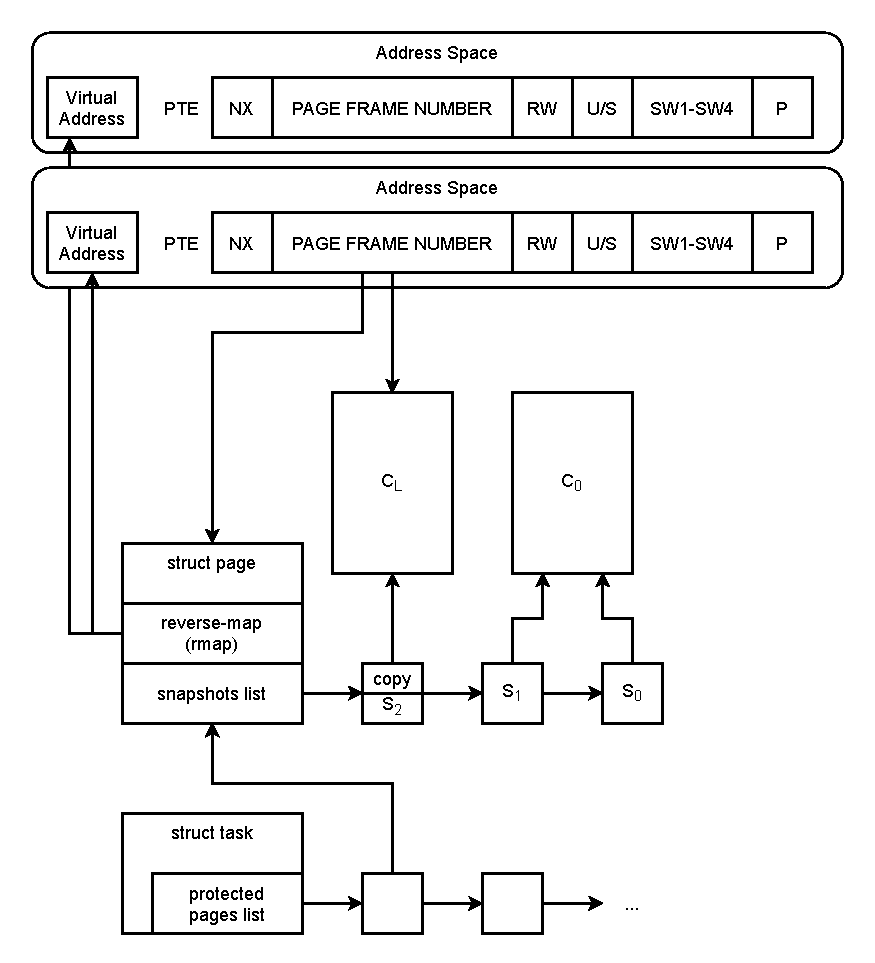
\includegraphics[width=\linewidth]{img/book-keeping.pdf}
  \caption{The most important marking information on x86}
  \label{fig:bookkeeping}
\end{figure}



\section{Related Work}
\label{sec:relatedwork}
Literature related to TikTok can be broadly divided in 2 groups. The first group
are system call wrappers and filters whose main vulnerability TikTok is
mitigating. The second one are the mitigations and solutions for double-fetches,
which are a superclass of TOCTTOU bugs. We discuss both groups in this section
and describe the benefits TikTok brings to the first group, and the advantages
over the second group.

\subsection{System Call Wrappers and Filters}

Watson in \cite{watson2007exploiting} scrutinized the security of many system
call wrappers. Not only that he found that all of them were insecure, Watson
described the different types of TOCTTOU bugs and discussed potential fixes.
In a short paragraph he mentions that Pawel Dawidek, the creator of CerbNG 
\cite{zak_frasunek_dawidek}, has experimented with marking arguments read-only.
CerbNG was an early system call filtering system for BSD that used copying to 
protect the arguments. To our knowledge nothing came out of those experiments. 
\\
\\
Afterward, Watson briefly discusses problems the such memory marking systems
need to solve: 
\begin{itemize}
    \item unnecessary page-faults
    \item bypassing memory marking using IO system calls
    \item mapping shared memory late
    \item handling system calls that write to memory correctly
\end{itemize}

TikTok addresses all of these issues. Unnecessary page-faults are rare and they
are used to make the offending threads wait for unmarking. After the page has
been unmarked, the write proceeds without any consequences. Write system call
does not proceed until there are no marked pages of the file. If needed, pages
are marked when they are mapped. TikTok also postpones all writes to marked
pages coming from kernelspace, while allowing the system calls to execute
correctly.
\\
\\
Modern system call wrappers can be classified in two groups, based on how they
approach the TOCTTOU attack. The first group eliminates all functionality
vulnerable to the attack.
Linux's \emph{SecComp}\cite{seccomp} and \emph{eBPF}\cite{ebpf} belong to this
group. The second group moves the filter checks deeper into the system calls,
eliminating the need to read the arguments twice. \emph{Landlock Linux}
\cite{landlock} and Google's \emph{Kernel Runtime Security Instrumentation}
(KRSI)\cite{krsi} embrace this technique.

\subsubsection{Partial Solutions}
SecComp\cite{seccomp} uses \emph{Berkeley Packet Filter} (BPF) to provide small,
programmable filters that execute before the system call. Based on the values
in registers, Linux can decide whether to allow, or to prevent a system call.
However, BPF cannot dereference pointers because an adversary would by able to
bypass those checks using a TOCTTOU attack. \emph{Extended Berkeley Packet
Filter} (eBPF)\cite{ebpf} provides larger filters which can also dereference
user pointers. However, eBPF cannot be used for security purposes - it cannot
stop system calls from executing. EBPF is completely read-only and can only be
used for tracing.
\\
\\
\subsubsection{LSM-based Solutions}
Landlock\cite{landlock} and KRSI\cite{krsi} use \emph{Linux Security Module}
\cite{morris2002linux} (LSM) hooks to call filter checks after the arguments
have already been copied into the kernel. LSM hooks have been imagined as a set
of places where arbitrary checks can be performed before accessing a kernel
resource. Execution proceeds only if the execution has been successful.
Different security modules can provide different hooks to provide different
guarantees (e.g. \emph{SELinux}\cite{smalley2001implementing} and
\emph{AppArmor}\cite{gruenbacher2007apparmor}).
\\
\\
Both Landlock and KPSI attach eBPF filters to hooks, allowing users to provide
custom rules for system calls. For this solution to work everywhere for perfect
syscall filtering, LSM hooks would need to be manually added to all Linux
drivers and ioctls. Unfortunately, this is highly impractical and requires a
considerable effort from a large group of developers. Considering that LSM
focuses on access control to kernel objects, it is questionable if an LSM module
can be used to mitigate bugs based on the system call arguments. Some of the
bugs could manifest themselves before a hook has been executed. TikTok is a
generic solution that does not require modifying the drivers, nor the use of
LSM hooks. Once it is deployed, all double-fetch bugs are eliminated from all
the drivers. A system call wrapper that uses TikTok can be completely
independent from the implementation of the system calls it is filtering.

\subsection{Double-Fetch Solutions}

Solutions for double fetch bugs can be divided into \emph{static} and
\emph{dynamic} techniques. Static techniques do not execute the program, but
analyze the source code. Dynamic techniques analyze the execution of the
program to find any violations.

\subsubsection{Static Analysis Work}
\label{subsec:dfstatic}
Static analysis techniques analyze the source code to find double-fetch bugs.
Wang et al. \cite{wang2017double} used pattern matching to find potential
double-fetches. They implemented a tool that patches certain double fetches
automatically. However, their method in the general case produces false
positives which need to be inspected manually. Xu et al.\cite{xu2018precise}
improved on this work by proposing Deadline. Deadline does not use the pattern 
analysis on the source files to detect double fetches, but a compiler's
intermediate representation and constraint solving to eliminate false positives.
\\
\\
Static analysis techniques such as these have the benefit of being able to find
bugs in the code that we cannot actually run (e.g. we are missing hardware to
test the drivers). However, they are meant for bug detection, not mitigation.
Even though the tools can fix some bugs automatically, this is not always
possible. The TOCTTOU bug is in system call wrappers by design. Another problem
are the double fetches which are not visible in the source, nor in the
intermediate representation. Compilers can introduce such invisible double
fetches when allocating registers to variables. TikTok is a mitigation technique
that works even in such cases.
\\
\\

\subsubsection{Dynamic Analysis Work}
Google Project Zero's Bochspwn \cite{jurczyk2013bochspwn} uses an emulator to
detect double-fetches. It found an quite a large number of bugs in the Windows
kernel. Bochpwn works on binaries, does not require access to the source code
and it detects bugs introduced by compilers. However, it is also limited to the
detection of double-fetches. Similarly to work prestented in 
\cref{subsec:dfstatic}, developers need to manually fix the bugs. However, with
dynamic analysis a double fetch also needs to be executed, limiting this
techniques to the core kernel and to the drivers with the available hardware.
\\
\\
A big leap in dynamic analysis techniques has been presented by Schwartz et al.
\cite{schwarz2018automated}. The first part of the paper introduces DECAF - a
framework that uses side-channel attacks to create a fuzzing oracle for
double-fetch bugs. While Bochspwn relies on emulation, slowing it down
significantly, DECAF runs natively. It also eliminates false positives by
automatically exploiting found bugs.
\\
Schwartz et al. then discuss a real-time mitigation technique for double
fetches - DropIt. DropIt uses Intel's \emph{Transactional Synchronization 
Extensions} (TSX)\cite{intel64and} in a creative way to prevent double fetch
bugs. By encapsulating the code in a TSX transaction, writes from other threads
to the addresses we have previously read from or written to will result in the
transaction being aborted. However, the code executing inside a TSX transaction
is severly limited. All reads must fit in the L3 cache, and all writes in L1,
with some instructions being forbidden. TikTok has none of those limitations.
It works on non-Intel processors and relies on page tables for protection - a
technique which has been present for several decades.


%-------------------------------------------------------------------------------
\section*{Acknowledgments}
%-------------------------------------------------------------------------------

Thanks, mom!

%-------------------------------------------------------------------------------
\section*{Availability}
%-------------------------------------------------------------------------------

The source code of TikTok is available at LINK. It has been released under the
GNU Public Licence.

%-------------------------------------------------------------------------------
\bibliographystyle{plain}
\bibliography{\jobname}

%%%%%%%%%%%%%%%%%%%%%%%%%%%%%%%%%%%%%%%%%%%%%%%%%%%%%%%%%%%%%%%%%%%%%%%%%%%%%%%%
\end{document}
%%%%%%%%%%%%%%%%%%%%%%%%%%%%%%%%%%%%%%%%%%%%%%%%%%%%%%%%%%%%%%%%%%%%%%%%%%%%%%%%

%%  LocalWords:  endnotes includegraphics fread ptr nobj noindent
%%  LocalWords:  pdflatex acks
